%!TEX root = ../D3.5_Examples_Compendium_2.tex
\section{Unmanned Aerial Vehicle}
\label{sec:uavsingle}

	\subsection{Example Description}
	\label{sec:uavsingle_desc}
		This pilot study originates from a master thesis study presented in \cite{Grujic&16}.
		The study models the physical dynamics as well as the discrete controller of an Unmanned Aerial Vehicle (UAV).
		Focus on the details of the model contribute to a high model fidelity, enabling the multi-model to be used to compare alternative control algorithms.

		\autoref{fig:uav_3d_model} shows a 3D model of the UAV and some of its main components, including the \texttt{airframe}, which is the main body the UAV, the propulsion system consisting of \texttt{rotors}, \texttt{motors}, and \texttt{electronic speed controllers}, along with the \texttt{battery} and the \texttt{controller} platform.
		Additionally, a UAV have a range of different \texttt{sensors} and a \texttt{telemetry system} used to communicate with a pilot or a ground control center.

		\begin{figure}[htbp]
			\centering
			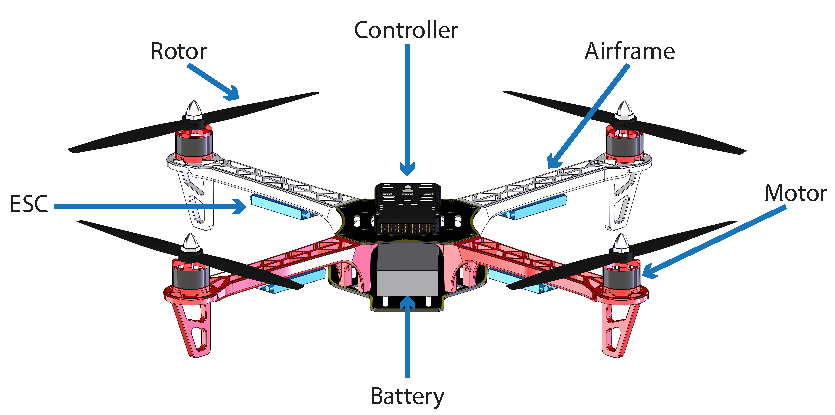
\includegraphics[width=0.7\linewidth]{uavsingle/drone.pdf}
			\caption{UAV 3D model}
			\label{fig:uav_3d_model}
		\end{figure}

	\subsection{Usage}
	\label{sec:uavsingle_usage}
		The example is available from the INTO-CPS application menu at \emph{File>Import Example Project} or at  \url{https://github.com/into-cps/case-study\_UAV} in the \emph{master} branch. There are several subfolders for the various elements: \texttt{FMU} -- contains the various FMUs of the study; \texttt{Models} -- contains the constituent models defined using the INTO-CPS simulation technologies; \texttt{Multi-models} -- contains the multi-model definitions and co-simulation configurations -- with 3D and non-3D options; and \texttt{SysML} -- contains the SysML model defined for the study.

		In the \emph{abstract\_intocps} branch, the original discrete event control model have been replaced with an abstract control model in order to enable high-level control prototyping.
		A prototype of an autonomous vertical waypoint controller is exemplified.
		The same model is found in the \emph{abstract\_crescendo} branch, where DESTECS technology is used instead of INTO-CPS technology.
		This can be used to compare the two technologies \cite{Thule&16b}.

	\subsection{INTO-CPS SysML profile}
	\label{sec:uavsingle_into_sys}
		The INTO-CPS SysML profile is used to create an Architecture Structure Diagram (ASD) and a Connections Diagram (CD), shown in \autoref{fig:uav_architecture_diagram} and \autoref{fig:uav_connections_diagram} respectively.
		The ASD expresses that the system \texttt{UAV} is a composition of a cyber part \texttt{ArduPilot}, a physical part \texttt{ArduCopter}, and an optional \texttt{3D animation}.

		\texttt{ArduPilot} is a discrete event controller described in VDM-RT. 
		It takes a number of sensor inputs and outputs a control signal for each of the four motors of the UAV.
		By adjusting the motor setpoints, it is able to make the UAV fly to predefined waypoints, taking into account feedback from sensors.

		\texttt{ArduCopter} is a model of the physical dynamics of the UAV described in 20-sim.
		The inputs to the \texttt{ArduCopter} model are the four motor setpoints. 
		Based on these, it calculates the angular position described with roll, pitch, and yaw angles, and the spatial position described with a latitude, longitude, and altitude (X,Y,Z), and the velocities and accelerations of the UAV.
		Additionally, corresponding sensor outputs are simulated for a 3-axis accelerometer, a 3-axis gyroscope and a GPS. 
		
		Angular and spatial positions are used by the \texttt{3D animation}.

		\begin{figure}[htbp]
			\centering
			\includegraphics[width=\linewidth]{uavsingle/architecture_diagram.png}
			\caption{UAV Architecture Structure Diagram}
			\label{fig:uav_architecture_diagram}
		\end{figure}

		The connection between the constituent models is a one-to-one mapping between \texttt{ArduPilot} and \texttt{ArduCopter}, with the exception that the \texttt{3D animation} is connected to \texttt{ArduCopter} as well, as shown in \autoref{fig:uav_connections_diagram}.
		

		\begin{figure}[htbp]
			\centering
			\includegraphics[width=\linewidth]{uavsingle/connections_diagram_3d.png}
			\caption{UAV Connections Diagram}
			\label{fig:uav_connections_diagram}
		\end{figure}


	\subsection{Multi-model}
	\label{sec:uavsingle_into_mm}

	\subsubsection{Models}
		The system comprises a continuous-time (CT) model \texttt{ArduCopter} and a discrete event (DE) model \texttt{ArduPilot}.
		\begin{description}
			\item[ArduCopter:] 
				The physical dynamics of the UAV is described in 20-sim.
				In \autoref{fig:uav_20-sim_model} an overview of the \texttt{Quadcopter} model is shown.
				It includes the rigid body dynamics of the \texttt{airframe}, the aerodynamics of the \texttt{rotors}, the electronics and mechanics of the \texttt{motors} and the \texttt{electronic speed controllers}, as well as \texttt{sensor} noise, inaccuracies, and rounding errors. 
				\begin{figure}[htbp]
					\centering
					\includegraphics[width=\linewidth]{uavsingle/ct_model.png}
					\caption{20-sim model of the UAV}
					\label{fig:uav_20-sim_model}
				\end{figure}

			\item[ArduPilot:]
				\autoref{fig:uav_ardupilot_overview} shows an overview of the \texttt{ArduPilot} model, which is described in VDM-RT.
				The main class of the model \texttt{ArduPilot} starts a \texttt{Scheduler} and a \texttt{Flight controller}.
				To improve model fidelity, sensor values are updated periodically by the scheduler to emulate the real update frequencies of the various sensors.
				The flight controller takes input from a pilot and from sensor data, on which sensor fusion is performed, and is responsible for calculating desired accelerations for the UAV. 
				These accelerations are translated, by the \texttt{Motors} class, into motor setpoints for each motor.
				The translation involves a complex tradeoff between roll, pitch, and yaw accelerations and total thrust.
				The \texttt{MotorsQuad} class is shown to illustrate that the \texttt{Motors} class can be extended to support any number or configuration of motors.

				The \texttt{Flight Control} class contains the core functionality of the model and is probably also the most complex part.
				It can operate in multiple flight modes, which make use of either an attitude controller or both an attitude and a position controller.
				The attitude controller is capable of obtaining and maintaining any given attitude, whereas the position controller is capable of controlling the altitude.
				Both the attitude and position controllers depend on a number of low level controllers, such as Proportional-Integral-Derivative (PID) controllers and a number of different filters to remove unwanted noise and vibrations caused by the fast spinning rotors.
				\begin{figure}[htbp]
					\centering
					\includegraphics[width=\linewidth]{uavsingle/detailed_de_model.png}
					\caption{ArduPilot model overview}
					\label{fig:uav_ardupilot_overview}
				\end{figure}

		\end{description}
		
	\subsubsection{Configuration}
		This pilot study does not use any parameters and the connections should be self explanatory from \autoref{fig:uav_connections_diagram}.

	\subsection{Co-simulation}
	\label{sec:uavsingle_into_co}
		Two multi-models are defined for this pilot study.
		The only difference between the two is whether the 3D animation is included or not.

		\begin{figure}[htbp]
			\centering
			\includegraphics[width=0.5\linewidth]{uavsingle/drone_animation_cropped.png}
			\caption{3D visualization of the UAV}
			\label{fig:uav_3d_animation}
		\end{figure}